\documentclass[a4paper,12pt]{report}
\usepackage{amsmath,amssymb,amsthm,latexsym,enumerate}
\usepackage{caption}
\usepackage{subcaption}
\usepackage[dvips]{graphicx}
\graphicspath{{./images/}}
\usepackage[dvips]{rotating}
\usepackage{curves}
\usepackage{color}
\usepackage{epic}
\usepackage{tikz}
\usetikzlibrary{automata, positioning}
\usepackage{hyperref}
\usepackage[natbib,backend=biber,style=authoryear]{biblatex}
\addbibresource{references.bib}

\textwidth 16.5cm
\oddsidemargin 0cm
\evensidemargin 0cm
\textheight 24cm
\topmargin -2cm
\parskip 0cm
\parindent 1cm

\theoremstyle{plain}
\newtheorem{theorem}{Theorem}[chapter]
\newtheorem{lemma}[theorem]{Lemma}
\newtheorem{conj}[theorem]{Conjecture}
\newtheorem{cor}[theorem]{Corollary}
\newtheorem{prop}[theorem]{Proposition}

\def\endmark{\hskip 2em$\square$\par}
\def\proof{\trivlist \item[\hskip \labelsep{\bf Proof\ }]}
\def\endproof{\null\hfill\endmark\endtrivlist}

{\theoremstyle{definition}
\newtheorem{definition}[theorem]{Definition}
\newtheorem{example}[theorem]{Example}
\newtheorem{notation}[theorem]{Notation}
\newtheorem{remark}[theorem]{Remark}
\newtheorem{algorithm}[theorem]{Algorithm}
\newtheorem{note}[theorem]{Note}
\newtheorem{question}[theorem]{Question}}

\newcommand*{\expect}{\mathbb{E}}
\newcommand*{\prob}{\mathbb{P}}
\newcommand*{\sigalgebra}{\mathcal{F}}

\title{\Huge Hidden Markov Models}
\author{Diljeet Jagpal}
\date{Spring 2021}

\begin{document}

    \maketitle

    \chapter*{Preface}
    \label{Abstract}
    Hidden Markov Models (HMM) allow us to explain some black-box systems, where we only have access to the observation, and the underlying system assumed Markovian. In this project, we seek to decide if these models provide any value in explaining the black-box system of rainfall.

We begin by replicating existing models by Cowperthwait and Grando to establish the known ability of HMM in rainfall simulation. We then provide an alternative approach to existing rainfall HMM parameter estimation, applying Baum-Welch to a discretised dataset. Finally, we attempt to generalise the model by generalising the HMMs observation matrix into a function of random variables.

We produce simulations using the HMM and the generalised HMM and compare, both graphically and numerically, the simulations to our dataset. 

While our function used for generalising was not successful, the HMM showed potential when compared to both test and training datasets.

All files are available at \href{https://github.com/djagpal02/HiddenMarkovModels_RainGenerators }{https://github.com/djagpal02/HiddenMarkovModels\_RainGenerators}.

	\pagenumbering{roman}
	\tableofcontents

	\newpage
	\pagenumbering{arabic}

	\chapter{Introduction}
    \label{Introduction}
	The goal of this project is to determine if HMMs are suitable as rain generators.

The first task will be to extend on the work done by Grando. In her testing, she has come to the conclusion that HMMs are suitable as rain generators however she has used the same data for testing as she used for training. This, quite likely, has lead to bias and thus we will extend her work by conducting out-of-sample tests. 

If possible, I will build the software so it is user friendly and efficient. With this, I can test data for multiple locations. This will allow me to understand if the result is truly signficant, at least more so than just one location.
	\newpage

	\chapter{Hidden Markov Models}
	\label{Hidden_Markov}
	In this section, we will briefly visit the foundations on which we will build throughout this paper. For most, this will be a simple refresher.

\section{Mathematical Foundations}
We start with a few key mathematical concepts.
\subsection{Probability Theory}
To discuss any probabilistic ideas we must first understand general probability theory. This can be done through the definition of a probability space.
\begin{definition}
	\label{probtheory}
	Probability Space \\
	A probability space is defined by $(\Omega ,\sigalgebra , \prob)$. $\Omega$ is the non-empty set of 		all possible outcomes, such that all events $\omega$ $\in$ $\Omega$. $\prob$ is a probability				measure, a function $\prob$(A) that maps event A to a number within [0,1] based on the liklihood of 		the event. $\sigalgebra$ is a $\sigma$-algebra on $\Omega$ if

	\begin{enumerate}
		\item $\Omega$ $\in$ $\sigalgebra$
		\item A $\in$ $\sigalgebra$ implies $A^c$ $\in$ $\sigalgebra$
		\item if $A_1, A_2, A_3$,... are in $\sigalgebra$ then so is $A_1 \cup A_2 \cup A_3$...
	\end{enumerate}
\end{definition}

\subsection{Conditional Probability}
Sometimes we require the probability of an event assuming another event has occured. In such situations we require conditional probability. Given two events A and B, the probability of event A occuring conditioned on the occurance of event B can be calculated as below. \\ 
\begin{equation}
\label{condprob}
	\prob (A|B) = \dfrac{\prob (A \cap B)}{\prob (B)}, \  \forall A \in \sigalgebra
\end{equation}
\\

From \ref{condprob} and the fact that for dependednt events $\prob$(A $\cap$ B) = $\prob$(B $\cap$ A) we can see that:

\begin{equation}
\label{intersection}
	\prob (A \cap B) = \prob (A|B) \prob (B) = \prob (B|A) \prob (A), \  \forall A,B \in \sigalgebra
\end{equation}
\\

Subsituting \ref{intersection} into \ref{condprob} we get the famous Bayes Theorem. 

\begin{theorem}
\label{bayes}
	Bayes’ Theorem \\
	For dependent events A and B with probability space $(\Omega ,\sigalgebra , \prob)$ , where $\prob$			(B) $\ne$ 0,
	\begin{equation}
		\prob (A|B) = \dfrac{\prob (B|A) \prob (A)}{\prob (B)}, \  \forall A \in \sigalgebra
	\end{equation}
\end{theorem}



\subsection{Stochastic Process}
To be able to define a Markov model, of any kind, we must first define a stochastic process. 
\begin{definition}
\label{stochasticp} 
	Stochastic Process \\
	Given an ordered set T and probability space $(\Omega ,\sigalgebra , \prob)$ a stochastic process is 		a collection of random variables X = \{$X_t$; t$\in$T\}. Based on t $\in $ T and $\omega \in \Omega$ 		we get a numerical realization of the process.  For simplicity, this may be viewed as a function; 			$X_t( \omega)$.

\end{definition}




\section{Applied Foundations}

	\newpage

	\chapter{Model Selection}
    \label{Model_Selection}
	\section{History}
Andrei Markov discovered the Markov model while analyzing the relationship between consecutive letters from text in the Russian novel "Eugene Onegin". With a two state model (states Vowel and Consonant) he proved that the probabililty of letters being in a particular state are not independent. Given the current state he could probabilistically predict the next. This chain of states, with various probabilities to and from each state, formed the foundation of the Markov Chain.

\section{Markov Chain}
A Markov chain is a network of connceted states. At any given time the model is said to be in a particular state. At a regular discrete interval the model has the ability to change states, which state will depend on the probaility and randomness. To define a Markov chain we must first address the Markov property. This simply states that the next state depends only on the current state. A more formal definition is given below. 

\begin{definition}
\label{markovproperty}
	Markov Property \\
	Let \{$X_t$ ; t $\in \mathbb{N}_0$\} denote a stochastic proccess \ref{stochasticp}, where t represents discrete time. The process has the Markov property if and only if,
	\begin{equation}
		\prob \{X_{n+1} = i_{n+1} | X_n = i_n, X_{n-1} = i_{n-1},...,X_0 = i_0\} = \prob \{X_{n+1} = 				i_{n+1} | X_n = i_n\}
	\end{equation}
\end{definition}


A Markov chain is simply a model that obeys \ref{markovproperty}. Again a more formal definition is given below.

\begin{definition}
\label{markovchain}
	Markov Chain \\
	A stochastic process \{$X_t$ ; t $>$ 0\} is a Markov Chain if and only if it satisfies the Markov property \ref{markovproperty}.
\end{definition}

To store the sequence of states a Markov chain has been through, we use the set $Q = \{q_t ; t \in \mathbb{N}_0\}$, where $q_t$ represents the state at time $t$. We will use this notation throughout the paper.

\begin{example}
	\label{stateseq}
	Given a Markov Model with states S = $\{S_1,S_2,S_3\}$, if the model starts at $S_2$ and then goes to $S_3$ and then back to $S_2$ the state sequence $Q$ will be $Q = \{q_1 = S_2, q_2 = S_3, q_3 = S_2\}$.
\end{example}

From the markov property we can see that the only thing that influences $q_t$ is $q_{t-1}$. Thus we can make a prediction for $q_{t+1}$ based on the outward transition probabililties from state $q_t$. If we calculate the probability of all possible states $S_j$ and use a biased random variable we can make a prediction.
\\
i.e. 
\\
Given a Markov chain with N states including $i$ and $j$ and discrete time $t \in \mathbb{N}_0$:
\begin{equation}
	\prob (q_t = S_j | q_{t-1} = S_i)_{1 \leq i,j \leq N}
\end{equation}


These probabilities can vary with time but can become quite complex. Thus, we usually assume the probabilities are constant. These special Markov models are called time-homogenous. 

\begin{definition}
\label{timehomogenous}
	Time homogenous \\
	Let \{$X_t$ ; t $\in \mathbb{N}_0$\} denote a stochastic proccess \ref{stochasticp}, where t represents discrete time, and $p(i,j)$ represent the transition probability from state i to state j. If 
	\begin{equation}
		\prob \{X_n = j | X_{n-1} = i\} = p(i,j),       \forall n \in \mathbb{N}_0
	\end{equation}
	then the process is time-homogenous.
\end{definition}

For a discrete Markov model with N states, there are N$^2$ possible transitions, where $p(i,j) = 0$ represents an impossible transition. We must store each of these probabilities. Given a time-homogenous Markov chain, we can create a 2-dimensional N x N matrix of transition probabilities $p$. Unique Markov chains have unique transition matrices. These matrices can be defined as below:

\begin{equation}
	\label{pmat}
	p = \{ p(i,j) = \prob \{ X_n = j | X_{n-1} = i \}\}_{1 \leq i,j \leq N}
\end{equation}

All $p$ matrices have some special characteristics. The first, is that all values contained within $p$ must be within $[0,1]$. This is quite natural as all values are probabililties and thus by definition must lie within $[0,1]$. The second is that all either the rows, columns or both form stochastic vectors. If it is the rows then the matrix is defined as a right-stochastic matrix, if it is the columns then it is called a left-stochastic matrix.\\

To demonstrate we will present an example where the weather is represented by the states.  

\begin{example}
\label{weathermarkovchain}
	Let \{$X_t ; t \in \mathbb{N}_0$\} denote a Markov Chain, with state space S = \{rainy, sunny, cloudy\}, where t represents the number of days from start. Since any state can transition into any other state, we say this model is ergodic. This can also be seen through the figure below as each state is connected to all others. 
	
	\begin{center}
	\begin{tikzpicture}
        \node[state] at(-3,0) (s) {Sunny};
        \node[state] at(3,0)  (r) {Rainy};
        \node[state] at(0,-3)  (c) {Cloudy};

        \draw[every loop]
            (s) edge[bend right=20, auto=left] node {0.4} (r)
            (s) edge[bend right=20, auto=right] node {0.2} (c)
            (s) edge[loop left] node {0.4} (s)       
            (r) edge[bend right=20, auto=left] node {0.4} (c)
            (r) edge[bend right=20, auto=right] node {0.3} (s)
            (r) edge[loop right] node {0.3} (r) 
            (c) edge[bend right=20, auto=right] node {0.5} (r)
            (c) edge[bend right=20, auto=left] node {0.2} (s)
            (c) edge[loop below] node {0.3} (c);
	\end{tikzpicture}
	\\
    In this Markov Chain diagram, as per usual, the arrows indicate the transition between states and the values next to these correspond to the probability of this transition. 
	\end{center}
\end{example}

Using \ref{weathermarkovchain} we can create a matrix $p$. To make this clear, we first create a table with our states labeled for rows and columns, where the $p(i,j)$ is the cell corresponding to row $i$ and column $j$.

\begin{center}
	\begin{tabular}{c c c c}
		x      & Sunny & Rainy & Cloudy \\
		Sunny  & 0.4   & 0.4   & 0.2 \\
		Rainy  & 0.3   & 0.3   & 0.4 \\ 
		Cloudy & 0.2   & 0.5   & 0.3 
	\end{tabular}
\end{center}

This content of this table forms the matrix $p$. 

\begin{equation}
p = 
\begin{bmatrix}
	0.4 & 0.4 & 0.2 \\
	0.3 & 0.3 & 0.4 \\
	0.2 & 0.5 & 0.3 
	\end{bmatrix}
\end{equation}

Now that we have a Markov Model with its $p$ we must reflect on its potential uses. Some natural questinos one may ask are:
\begin{enumerate}
	\item Given at time $t$ the state was $S_i$, what is the most likely state time $t+1$?
	\item What is the probability of getting a particular state sequence $O$?
	\item What is the probability of staying within a state for d time steps?
\end{enumerate}

This first problem can be addressed simply using the matrix $p$. Our motivation behind it was to build a matrix where $p_{ij}$ contains the probability of moving from $i$ to $j$. Thus, we can simply look at the current row and find the largest probability and its corresponding $j$.
\begin{example}
	Let us refer back to \ref{weathermarkovchain} and assume the current state is Cloudy. We can see that 0.2 $<$ 0.3 $<$ 0.5 and that 0.5 corresponds to Rainy. Thus our the most likely next state would be Rainy. 
	\\
	If the current state was sunny, we would have two maximums of 0.4. In such case, the process is equally likely to go to either. 
\end{example}

The second problem provides a state sequence $Q = \{q_t,q_{t+1},q_{t+2}...\}$ and asks what the probability of this occuring is, i.e. $\prob (Q | model)$. This can be simplified quite easily as shown below.
\begin{eqnarray}
	\label{markovchainstateseqprob}
	\prob (Q | model) & = & \prob (\{q_t,q_{t+1},q_{t+2}...\} | model) \\
					  & = & \prob (q_{t}) \prob (q_{t+1}| q_{t}) \prob (q_{t+2}| q_{t+1})... \\
					  & = & \prob (q_t) p(q_t,q_{t+1}) p(q_{t+1}q_{t+2}) ...
\end{eqnarray}

\begin{example}
	We can now use \ref{markovchainstateseqprob} to demonstrate the probability of a state squence from \ref{weathermarkovchain}. Let $Q = \{$Sunny, Sunny, Cloudy, Rainy\}. Given that we start from Sunny: 
	\begin{eqnarray}
		\prob (Q | model) & = & \prob (\{Sunny, Sunny, Cloudy, Rainy\} | model) \\
						  & = & \prob (Sunny) \prob (Sunny| Sunny) \prob (Cloudy| Sunny) \prob (Rainy| Cloudy)\\
						  & = & 1 * 0.4 * 0.2 * 0.5 \\
						  & = & 0.04 
	\end{eqnarray}
\end{example}

The third problem asks how long is the model likely to stay in any given state. Assume that the model stays in state $S_i$ for $d$ days. We can create a state sequence for this, $Q = \{q_t = S_i ,q_{t+1} = S_i, ..., q_{t+d-1} = S_i, q_{t+d} \neq S_i\}$.  Using the state sequence probabililty calculation from before we can compute the following equation:
\begin{equation}
	\prob (Q | model) = p(i,i)^{d-1} (1 - p(i,i)) = p_i(d)
\end{equation}

We label this $p_i(d)$ to represent the discrete probability density function of the duration d in state i. From this we can calculate the expected stay in any particular state. This is done using the following formula:
\begin{eqnarray}
	\label{expectedstay}
	\bar{d_i} & = & \sum_{d=1}^{\infty} d  p_i(d) \\
			  & = & \dfrac{1}{1 - p(i,i)}
\end{eqnarray} 

\begin{example}
	Reffering back to \ref{weathermarkovchain}, suppose we would like to see how many days in a row we expect it to be sunny. We see that $p(Sunny,Sunny)$ = 0.4. Now we can use \ref{expectedstay} to find, 
	\begin{eqnarray}
		\bar{d_{Sunny}} & = & \sum_{d=1}^{\infty} d  p_{Sunny}(d) \\
			  & = & \dfrac{1}{1 - p(Sunny, Sunny)} \\
			  & = & \dfrac{1}{1 - 0.4} \\
			  & = & 1.67
	\end{eqnarray}
	Thus we expect it to remain sunny for 1.67 days. Since we are dealing with discrete data, it is more approprate to round up to 2 days. 
\end{example}

The Markov model we have been discussing so far is called an observable Markov Model as we can observe its events. This is not always the case.


\section{Motivating the Hidden Markov Model}

Sometimes you do not get an observation from your states but only see the effect of the state change. To help develop this idea we borrow an example from \cite{1165342}.

\begin{example}
	\label{motivhmmcoin}
	Suppose there is someone hidden behind a barrier or curtain, where you cannot see what they are doing. This person is doing some kind of experiment with flipping coins and shouting heads or tails at regular intervals. You do not know:
	\begin{enumerate}[i]
		\item How many coins there are.
		\item If the coin/s is/are fair.
	\end{enumerate}
	Since the problem is quite vague, we must experiment with various models and see which fits the data the best. Since the only thing we can observe is the outcome, heads or tails, we will refer to this as our observation. Lets start with the simplest. 
	\begin{enumerate}
		\item 1-Fair Coin \\ In this model we have two states, heads and tails. There is a 0.5 probability for the model to change state and equally for staying in the same. The simplicity of this model comes at the cost of many assumptions that may not nessesarily hold true.
		\begin{center}
			\begin{tikzpicture}
				\node[state] at(-3,0) (H) {Heads};
				\node[state] at(3,0)  (T) {Tails};
				
				\draw[every loop]
					(H) edge[loop, auto=left] node {0.5} (H)
					(H) edge[bend right=20, auto=left] node {0.5} (T)
					(T) edge[loop, auto=left] node {0.5} (T)
					(T) edge[bend right=20, auto=left] node {0.5} (H);
			\end{tikzpicture}
			
			\begin{tabular}{c c}
		 		$\prob (Heads)$  & 0.5 \\
		 		$\prob (Tails)$  & 0.5  \\  
			\end{tabular}
		\end{center}
		\item 2-Fair Coin \\ This model also has two states but this time they reprsent two different coins. Both can produce heads and tails, thus we do not know which produced the observation. The fact that they are both Fair coins means that as an external observer, we will not be able to see a difference between this model and the 1-Fair Coin. However, it is clear that the observations are now independent of the hidden states transitions, as they are equally likely regardless of the state. In the 1-Fair Coin model we can determine perfectly which state the model is in from the observation, but this is no longer possible with this model.
		\begin{center}
			\begin{tikzpicture}
				\node[state] at(-3,0) (1) {Coin 1};
				\node[state] at(3,0)  (2) {Coin 2};
				
				\draw[every loop]
					(1) edge[loop, auto=left] node {0.5} (1)
					(1) edge[bend right=20, auto=left] node {0.5} (2)
					(2) edge[loop, auto=left] node {0.5} (2)
					(2) edge[bend right=20, auto=left] node {0.5} (1);
			\end{tikzpicture}
	
			\begin{tabular}{c c c}
				& $\prob (Coin 1)$ & $\prob (Coin 2)$ \\
		 		$\prob (Heads)$  & 0.5   & 0.5 \\
		 		$\prob (Tails)$  & 0.5   & 0.5 \\
			\end{tabular}
		\end{center}
		\item  2-Biased Coins \\ Although this model is similar to 2-Fair Coins, the change in $\prob (Heads)$ and $\prob (Tails)$ for each state has a large impact on the observation likelihood. It can be seen that if the model is in state 1 heads is more likely and if the state is in state 2 tails is more likely. As an observer we can now say if we see a tails, it was most likely from state 2 and if we see a heads, it was most likely from state 1. The change between these two states must be an unrealted proabbility, such as a third coin or another source of randomness.
		\begin{center}
			\begin{tikzpicture}
				\node[state] at(-3,0) (1) {Coin 1};
				\node[state] at(3,0)  (2) {Coin 2};
				
				\draw[every loop]
					(1) edge[loop, auto=left] node {0.5} (1)
					(1) edge[bend right=20, auto=left] node {0.5} (2)
					(2) edge[loop, auto=left] node {0.5} (2)
					(2) edge[bend right=20, auto=left] node {0.5} (1);
			\end{tikzpicture}
	
			\begin{tabular}{c c c}
				& $\prob (Coin 1)$ & $\prob (Coin 2)$ \\
		 		$\prob (Heads)$  & 0.75   & 0.25 \\
		 		$\prob (Tails)$  & 0.25   & 0.75 \\
			\end{tabular}
		\end{center}
		\item 3-Biased Coins \\ Similar to the 2-Biased Coins model, the probabilities for heads and tails vary with the three states.
		\begin{center}
			\begin{tikzpicture}
				\node[state] at(-3,0) (1) {Coin 1};
				\node[state] at(3,0)  (2) {Coin 2};
				\node[state] at(0,-3)  (3) {Coin 3};
		
				\draw[every loop]
					(1) edge[bend right=20, auto=left] node{} (2)
					(1) edge[bend right=20, auto=right] node{} (3)
					(1) edge[loop left] node{} (1)       
					(2) edge[bend right=20, auto=left] node{} (3)
					(2) edge[bend right=20, auto=right] node{} (1)
					(2) edge[loop right] node{} (2) 
					(3) edge[bend right=20, auto=right] node{} (2)
					(3) edge[bend right=20, auto=left] node{} (1)
					(3) edge[loop below] node{} (3);
			\end{tikzpicture}
			\begin{tabular}{c c c c}
				& $\prob (Coin 1)$ & $\prob (Coin 2)$ & $\prob (Coin 3)$\\
		 		$\prob (Heads)$  & 0.6   & 0.25 & 0.45 \\
		 		$\prob (Tails)$  & 0.4   & 0.75 & 0.55 \\
			\end{tabular}
			\end{center}
	\end{enumerate}
\end{example}

An important conclusion one may make, after contemplating which model is best, is that it is quite difficult to decide on how many states are needed without priori information. In such case, we must ensure that there are enough states, such that the model does not over generalize but also not so many that it requires to much data to train. Naturally, one would assume choosing the larger number of states is more suitable as they can take the shape of a model with fewer states but the opposite is not true. However, larger models require much more data to be statisticaly reliable as there are alot more uknown variables that must be found. Below we show this for our models, along with where the uknowns come from (-s being from the state transition proabilities and -O being from the observation probabililties). 

\begin{center}
	\begin{tabular}{c c c}
		Model  & Number of Unknowns & From\\
		1-Fair Coin    & 0 & - \\
		2-Fair Coins   & 1 & 1-S\\ 
		2-Biased Coins & 4 & 2-S 2-O\\
		3-Biased Coins & 9 & 6-S 3-O
	\end{tabular}
\end{center}

Hence, the best approach is usually to base the model state size on the amount of available data. This is not always garenteed to give reliable results but can sometimes be the only option, for example when limited by data.

The first model having 0 unknowns is also interesting. This is because here each state is linked with only one observation. Thus, as an observer, given an observation we can assert what state the model is in. This means the states are no longer hidden and the model is simply a standard markov model. 

Another important detail the avid reader may have noticed is in the case of 2-Biased Coins and 3-Biased Coins it is possible to make a reasonable guess of what state the model is in, i.e. which coin was flipped, based on the observation. Furthermore, the statistical properties of predictions generated using 1-Fair Coin and 2-Fair Coins should be identical but for 2-Biased Coins and 3-Biased Coins be somewhat unqiue. Due to this, unless the underlying system is completly fair, like in the first two, it should be possible to determine which model best fits the data, and thus determine the model.


This brings us to the core idea behind hidden markov models. Although we cannot directly observe the model or its properties, through sufficient observation data, we can attempt to create one that fits this data the best. 

	\newpage

	\chapter{Replicating Existing Rainfall Models}
	\label{Replicating_Existing_Rainfall_Model}
    \section{Definition}

A hidden markov model is a doubly stochastic markov process **citation**. This comes from the fact that there are two stochastic processes, one determining the transition between states and one determining the output observation. 

To define a hidden markov model we need 5 things.**citation**
\begin{enumerate}
    \item N \begin{enumerate}[i]
        \item N is the number of hidden states. This is usually based of something in the real world but sometimes can be uknown, as in \ref{motivhmmcoin}.
        \item The states are usually ergodic, i.e. from any given state you can reach another eventually but this is not nessesary.
        \item The states are from the state space $S = \{S_1,S_2,...,S_N\}$.
        \end{enumerate}
    \item M \begin{enumerate}[i]
        \item M is the number of observable outputs.
        \item These combine to make a discrete alphabet of observations called $V = \{v_1, v_2,...,v_M\}$.
    \end{enumerate}
    \item A \begin{enumerate}[i]
        \item A is the state transition matrix.
        \item This is the same as the $p$ matrix \ref{pmat}. 
        \item A = $\{a_{ij}\}$ 
        \item $a_{ij}$ = $\{ p(i,j) = \prob \{ X_n = j | X_{n-1}\}$
    \end{enumerate}
    \item B \begin{enumerate}[i]
        \item B is the observation probability matrix.
        \item B = $\{b_j(k)\}$
        \item $b_j(k) = \prob (V_k \  at \  t | q_t = S_j)_{1 \leq j \leq N, 1 \leq k \leq M}$
    \end{enumerate}
    \item $\pi$ \begin{enumerate}[i]
        \item $\pi$ is a vector containing all inital state probabilities. 
        \item $\pi$ = $\{ \pi_i \}$
        \item $\pi_i$ = $\prob (q_1 = S_i) for 1 \leq i \leq N$
    \end{enumerate}
\end{enumerate}

We can now combine the above to provide a formal definition of hidden markov models.
\begin{definition}
\label{hmm} Hidden Markov Model \\
A Hidden Markov Model is a 5-tuple $\{N,M,A,B,\pi \}$ that is used to represent a doubly stochastic process where the hidden process is markovian. 
\end{definition}

Before we continue we will also provide notation that will be used for the rest of the paper.
\begin{enumerate}[i]
    \item We will continue to use $Q$ \ref{stateseq} to represent the state sequence for markov model, i.e. the hidden process.
    \item We will use $O = \{O_1,O_2,...,O_T\} ,\ O_i \in V$ to represent the observation sequence.
    \item we will occasionally represent the hidden markov model as $\{N,M, \lambda \}$ where $\lambda = \{A, B, \pi\}$ 
\end{enumerate}


\section{Using HMM}
As with any mathematical model, we can use HMMs to predict future observations. As with simple markov models \ref{probmeas}, we can create probability measures but this time we must use conditioning. 

\subsection{Predictive Model}
 We can use HMM to generate a sequence of potential observations. Given a a hidden markov model, lets call it H = $\{N,M,A,B,\pi\}$, to generate a sequence of $T$ observations $O$ we do the following steps: **citation**
 \begin{enumerate}
    \label{hmmpredict}
     \item Using $\pi$ as a probability measure, set $t$ = 1 and randomly select a state as the first $q_1$ = $s_i$.
     \item Using $b_i(k)$ as a probability measure, randomly select the observation $O_t$ = $v_k$.
     \item Using $a_{ij}$ as a probability measures, set $t$ = $t+1$ and randomly select a the next state $q_{t+1}$ = $s_j$.
     \item Repeat steps 2 and 3 until $t$ = $T$
 \end{enumerate}

 To demonstrate this method, we will use an adapted version of \ref{weathermarkovchain}. This version will have the markov chain from before as the underlying hidden process and another process with state space \{Happy, Sad\}, which we can observe.

 \begin{example}
    \label{motivationhmm}
    Suppose Alice is hidden away from the world and has no access to information regarding the weather. She meets Bob everyday and knows how weather affects his mood.
    For simplicity, assume Bob only has two moods, happy and sad. Given matrix A, B and vector $\pi$ can she predict his mood for 3 consecutive days?
    \begin{figure}
        \centering
        \begin{tikzpicture}
            \node[state] at(-3,0) (s) {Sunny};
            \node[state] at(3,0)  (r) {Rainy};
            \node[state] at(0,-3)  (c) {Cloudy};
            \node at (-6,3) (h1) {Happy};
            \node at (-6,-3) (s1) {Sad};
            \node at (3,-6) (h2) {Happy};
            \node at (-3,-6) (s2) {Sad};
            \node at (6,3) (h3) {Happy};
            \node at (6,-3) (s3) {Sad};

            \draw[every loop]
                (s) edge[bend right=20, auto=left] node {0.4} (r)
                (s) edge[bend right=20, auto=right] node {0.2} (c)
                (s) edge[loop left] node {0.4} (s)       
                (r) edge[bend right=20, auto=left] node {0.4} (c)
                (r) edge[bend right=20, auto=right] node {0.3} (s)
                (r) edge[loop right] node {0.3} (r) 
                (c) edge[bend right=20, auto=right] node {0.5} (r)
                (c) edge[bend right=20, auto=left] node {0.2} (s)
                (c) edge[loop below] node {0.3} (c);
            
            \draw [->, dashed] (s) edge[auto=right] node{0.2} (s1);
            \draw [->, dashed] (s) edge[auto=right] node{0.8} (h1);
            \draw [->, dashed] (c) edge[auto=right] node{0.3} (s2);
            \draw [->, dashed] (c) edge[auto=right] node{0.6} (h2);
            \draw [->, dashed] (r) edge[auto=right] node{0.3} (s3);
            \draw [->, dashed] (r) edge[auto=right] node{0.7} (h3);
        \end{tikzpicture}
        \\
        The solid lines represent hidden probabilities and the dashed represent observable.
    \end{figure}
   \\
    From context we can deduce the following:
    \begin*{enumerate}
        \begin{center}
        \item N = 3, number of hidden states
        \item M = 2, number of possible observations
        \item \begin{equation}
            A = 
            \begin{bmatrix}
                0.4 & 0.4 & 0.2 \\
                0.3 & 0.3 & 0.4 \\
                0.2 & 0.5 & 0.3 
                \end{bmatrix}
            \end{equation}
        \item \begin{equation}
            B = 
            \begin{bmatrix}
                0.8 & 0.2 \\
                0.7 & 0.3 \\
                0.6 & 0.4 
                \end{bmatrix}
            \end{equation}
        \item \begin{equation}
            \pi = 
            \begin{bmatrix}
                0.5 \\
                0.3 \\
                0.2 
                \end{bmatrix}
            \end{equation}
        \end{center}
    \end*{enumerate}

    We can now use \ref{hmmpredict} to create an observation sequence $O$ = $\{o_1, o_2, o_3\}$. We will require multiple random variables generated using various different probability measures. I will these through python using my "rand.py" file. I will use a unifrom random variable. I will label these r.v.. I select the state that corresponds to the region on the cumulative probability distribution that the random variable lies on.
    \begin{enumerate}[i]
        \item We generate a r.v. = 0.0058. Using Pi as the probaility distribution, we select Sunny. We can now set $q_1$ = $s_1$.
        \item We generate a r.v. = 0.1947. Using $b_1(k)$ as the probability distribution we select Happy as the observation. We can now set $o_1$ = $v_1$.
        \item we generate a r.v. = 0.7168. Using $a_{1j}$ as the probability distribution we select Rainy as the next state. We now set $q_2$ = $s_2$.
        \item We generate a r.v. = 0.1060. Using $b_2(k)$ as the probability distribution we select Happy as the observation. We can now set $o_2$ = $v_1$.
        \item we generate a r.v. = 0.8977. Using $a_{2j}$ as the probability distribution we select Cloudy as the next state. We now set $q_3$ = $s_3$.
        \item We generate a r.v. = 0.1369. Using $b_3(k)$ as the probability distribution we select Happy as the observation. We can now set $o_2$ = $v_1$.
    \end{enumerate}
    Finally we can look back on our prediction $O$ and see that it is equal to $\{v_1,v_1,v_1\}$, i.e. we predict three consecutive Happy days.
\end{example}


\subsection{Three Key Problems}
There are many interesting questions one may pose regarding the HMM but there are three famous ones which we will focus on. Posed orgiinally by **citation**
\begin{enumerate}
    \item \label{q:first} Evaluation \\ Given model H = $\{N,M,A,B,\pi\}$ what is the probability that it generated the sequence of observations $O = \{o_1,o_2,...,o_T\}$? i.e. $\prob (O \ | \ H)$
    \item \label{q:second} Decoding \\ What sequence of states $Q = \{q_1, q_2,..., q_3\}$ best explains a sequence of observations $O = \{o_1,o_2,...,o_T\}$?
    \item \label{q:third} Learning \\ Given a set of observation $O = \{o_1,o_2,...,o_T\}$, how can we learn the model H = $\{N,M,A,B,\pi\}$ that would generate them?
\end{enumerate}

In the coming sections, for each problem, we will be motivating its uses and developing its solutions. 

\section{Problem 1: Evaluation}
Lets start by addressing question \ref{q:first}. Informally, we are looking for the proability that a given model generated a sequence of observations, i.e. $\prob (O | \lambda)$.

This probability has many useful applications. For example, you may have multiple potential models $\lambda_i$ and are unable to decide which one is the most suitable. In this case you can now calculate this probability for each $\lambda_i$ and the largest.

To find this probability we must consider the internal hidden states of the model. Since our probability of observations $\{b_j(k)\}$ is conditioned on the hidden state, we can start by calculating this probaility conditioned on these states. Lets assume we know what the state sequence $Q = \{q_1,q_2,...,q_t\}$ is. To $\prob (O | Q, \lambda)$ we can find the product of all the probabilities of an observation given the models state at all times $t$. In essence this breaks the  $\prob (O | Q, \lambda)$ into T parts. 
\begin{equation}
    \label{poq1}
    \prob (O | Q, \lambda) = \prod_{t=1}^T \prob (O_t | q_t, \lambda)
\end{equation}


An observation one may make is that these probabilities are simply taken from the matrix $B$. 
\begin{equation}
    \prob (O_t | q_t, \lambda) = b_{q_t}(O_t), \ \ \forall t \in [0,T] 
\end{equation}

Thus we can rewrite \ref{poq1} as:
\begin{equation}
    \label{oqlam}
    \prob (O | Q, \lambda) = b_{q_1}(O_1) b_{q_2}(O_2)  ...  b_{q_T}(O_T)
\end{equation}

Our next objective is to remove $Q$ from the conditioned part of the probability. To do this we must first calculate $\prob (Q | \lambda)$. This is simply the probability of transitioning from $q_1$ to $q_2$, $q_2$ to $q_3$ etc. More formally we can use matrix $A$ to find the probability of each of these transitions and since we are finding the total for the entire sequence, we just multiply them all togther. We start with $\pi_{q_1}$ as we also need the probability of starting at $q_1$.
\begin{equation}
    \label{qlam}
    \prob ( Q | \lambda) = \pi_{q_1} a_{q_1q_2} a_{q_2q_3} ... a_{q_{T-1}q_T}
\end{equation}

We can now successfully remove $Q$ from the condition using \ref{oqlam} and \ref{qlam}:
\begin{eqnarray}
    \label{oqgivenlam}
    \prob (O,Q | \lambda) & = & \prob(O | Q, \lambda) \prob(Q | \lambda) \\
                          & = & \pi_{q_1} b_{q_1}(O_1) a_{q_1q_2} b_{q_2}(O_2) a_{q_2q_3} ... a_{q_{T-1}q_T} b_{q_T}(O_T)
\end{eqnarray}

This gives us the joint probability of observations and the internal states. In other words, it provides the probabilty that given observations $O$ and internal state sequence $Q$ was generated by model $\lambda$. To achieve our desired probablity all we need to do is get rid of the $Q$. Since it is another input, all we must do is sum each value of \ref{oqgivenlam}. As we have accounted for every possible $Q$, we no longer need to worry about its particular value. This leaves us with:
\begin{eqnarray}
    \label{ogivenlamsumq}
    \prob (O | \lambda) & = & \sum_{all Q} \prob(O| Q,\lambda)P(Q|\lambda) \\
                        & = & \sum_{q_1,q_2,...,q_T} \pi_{q_1} b_{q_1}(O_1) a_{q_1q_2} b_{q_2}(O_2) a_{q_2q_3} ... a_{q_{T-1}q_T} b_{q_T}(O_T)
\end{eqnarray} 

Although this solution is correct, calculating this is infeasible. This is because it requires to many computations. For $T$ timesteps and $N$ states, to find every possible $Q$ we must sum over $N^T$ state sequences. For each timestep we require a multiplication to $a_{q_{i-1}q_{i}}$ and $b_{q_i}(O_i)$, except the last where there are no transitions. This leads to $2T-1$ multiplications for each state sequence. Lastly we require $N^T$ addition operations to sum the result for each state sequence. This gives us a final total number of operations of $(2T-1)N^T + (N^T-1)$. 

\begin{example}
    \label{motivfb}
    Lets refer back to \ref{motivationhmm}. Suppose we would like to find the probability of a string of 10 observations using model H. Here $N$ = 3 and $T$ = 10. 
    \begin{eqnarray}
        operations & = & (2T-1)N^T + (N^T-1) \\
                   & = & (20-1)3^10 + (3^10 -1) \\
                   & = & 1180979
    \end{eqnarray}
\end{example}


This is a problem as even with a smaller model \ref{motivfb} we require a very large number of calculations. For a moderate to large sized model we would require an infeasible amount of calculations. To overcome this problem we look for a more efficient method, the Forward-Backward algorithm.



\subsection{Forward-Backward Algorithm}
History of F-B , **citation**
The Forward-Backward algorithm (F-B) is composed of two helper functions $\alpha$ and $\beta$. We will start by discussing the former.

\begin{equation}
    \label{alpha}
    \alpha_t(i) = \prob (O_1,O_2,O_3,...,O_t,q_t=S_i | \lambda)
\end{equation}
$\alpha$ is an extremly powerful tool in reducing the number of calculations  **citation**. As given by \ref{alpha}, it providse the probability that at time $t$ we have seen a sequence of observations and are currently at state $q_t=S_i$. This is not quite $\prob (O | \lambda)$ but it represents a part of it. Instead of the probability of the whole sequence, it breaks it into a chunk of size $t$, commits to end at a particular state and then calculates the same proabbility for this.

We can combine \label{alpha} with induction to produce an iterative process that can calculate \ref{q:first}.

\begin{enumerate}[i]
    \item Base case \\
    For the base case we require the probability of the $q_1$ being equal to $S_1$ and giving us observation $O_1$. The former is addressed by $\pi_i$ and the later by $b_i(O_1)$. This gives us:
    \begin{eqnarray}
        \alpha_1(i) = \pi_i b_i(O_1), & i \in [1,N]
    \end{eqnarray}

    \item Inductive step: \\
    For the inductive step we must consider how to approach the next timestep. We will again be calculating for all $j\in [1,N]$ and as such must take into consideration, for each $j$, every possible $i$. This is again the same set of $[1,N]$. Therefore, to account for all possible previous states and their transition to the current state, we must sum over 1 to $N$ the product of $\alpha_t(i)$ and $a_{ij}$. For the given observation, as before, we compute $b_j(O_{t+1})$. Additionally, we must stop before reaching the final step as there is no outward transition and thus this would not be applicable. This gives us:
    \begin{eqnarray}
        \alpha_{t+1}(j) = \left[\sum_{i=1}^N \alpha_t(i)a_{ij}\right] b_j(O_{t+1}), & j \in [1,N], t \in [1,T-1]
    \end{eqnarray}

    \item Termination step: \\
    For the termination step we sum over all alpha at the final time $T$. Each alpha represents the probability of being in that given state at that particular time, through all possible sequences that it may have followed. Therefore, by summing all of these we now do not have to concern ourselves with the state sequence as all have been considered.
    \begin{eqnarray}
        \prob (O | \lambda) = \sum_{i=1}^N \alpha_T(i)
    \end{eqnarray}
\end{enumerate}

\begin{figure}
	\begin{center}
        \begin{tikzpicture}
            \node[state] at(-2,3) (s1) {$S_1$};
            \node[state] at(-2,1)  (s2) {$S_2$};
            \node at(-2,0)  (sd1) {.};
            \node at(-2,-0.5)  (sd2) {.};
            \node at(-2,-1) (sd3) {.};
            \node[state] at(-2,-2)  (sn) {$S_N$};
            \node[state] at(3,0) (new) {$S_j$};
            \node at(-2,-3) (a1) {$\alpha_t(i)$};
            \node at(3,-3) (a2) {$\alpha_{t+1}(i)$};
            \node at(-2,-4) (t1) {$t$};
            \node at(3,-4) (t2) {$t+1$};

            \draw [->] (s1) edge[auto=right] node{$a_{1j}$} (new);
            \draw [->] (s2) edge[auto=right] node{$a_{2j}$} (new);
            \draw [->] (sn) edge[auto=right] node{$a_{Nj}$} (new);
        \end{tikzpicture}
        \\
    For each state $j$, for each inductive step, we follow the above method. Each $\alpha_t(i)$ is multiplied by each $a_{ij}$ and then summed up. This result multipled by $b_j(O_{t+1}$ gives us $\alpha_{t+1}(j)$.
    \end{center}
\end{figure}



One can see that this method is far more efficient than \ref{ogivenlamsumq}. It requires $N^2$ multiplications for  $\alpha_t(i)$ and $a_{ij}$  for $T$ time periods. For each $T$ there are also $N$ addition operations for the summation and a multiplication for the $b_j(O_{t+1})$. This is true for all but the first and the last timestep, where there are $N$ multiplications and $N$ additions respectively. This gives us $(T-2)(N^2 + N + 1) + 2N$ calculations. Considering simply the order we see that the previous method had order $O(TN^T)$ whereas F-B gives us an order of $O(TN^2)$. It is now feasible to compute $\prob (O | \lambda)$.

\begin{example}
    \label{motivfb}
    We attempt to solve the problem \ref{motivfb} again but this time using the F-B algorithm. Suppose we would like to find the probability of a string of 10 observations using model H. Here $N$ = 3 and $T$ = 10. 
    \begin{eqnarray}
        operations & = & (T-2)(N^2 + N + 1) + 2N \\
                   & = & (10-2)(3^2 + 10 + 1) + 6\\
                   & = & 118
    \end{eqnarray}

    This is clearly many orders of mangitude smaller than 1180979, which was the requirement without F-B algorithm, thus it is a significant improvement. One may note, the improvement against the base method will be even more drastic for larger models, due to the $N^T$ term being removed.  
\end{example}


For question 1 this is sufficient. However, we will later require the $\beta$, the backward component and as such we will describe it now. Logically it is the same principle as the forward component except this time instead of moving forward step by step we are moving backwards.
\begin{equation}
    \label{beta}
    \beta_t(i) = \prob (O_{t+1},O_{t+2},,...,O_T | q_t=S_i, \lambda)
\end{equation}
This represents the probability of seeing the observations $O_{t+1}$ up to $O_T$ given that at time $t$ the model $\lambda$ is at state $S_i$. We again calculate this inductively.

\begin{enumerate}
    \item Base case \\
    For each state we must assume that it is the final state in order to iterate from it. This gives us:
    \begin{eqnarray}
        \beta_T(i) = 1, & i \in [1,N]
    \end{eqnarray}

    \item Inductive step: \\
    Each inductive step we move back by one timestep. As before, we will be calculating for all $N$ states except this time $i$ will be varying instead of $j$. This makes sense as we are stepping backward and we want to see which previous state is the most likely previous state. At each step, we the transaction probability of having coming from $i$, $a_{ij}$ to the probability of seeing the given observation at state $S_j$, $b_j(O_{t+1})$ and the liklihood of being at that state based on future states $\beta_{t+1}(i)$. This gives us:
    \begin{eqnarray}
        \beta_{t}(i) = \sum_{j=1}^N a_{ij} b_j(O_{t+1}) \beta_{t+1}(i), & i \in [1,N], t \in [1,T-1]
    \end{eqnarray}
\end{enumerate}



\section{Problem 2: Decoding}
We now turn our attention to \ref{q:second}. This problem is somewhat more difficult, as the definition of 'best' is quite vague and open to interpretations. An obvious appraoch would be to look for the states that are individually most likely for each state for a set time $t$ given all observations and the model. Lets define this probaility as $\gamma$.
\begin{equation}
    \gamma_t(i) = \prob (q_t = S_i | O, \lambda)
\end{equation}

Using \ref{alpha} and \ref{beta} we can solve for $\gamma$ quite quickly. If we recall, $\alpha_t(i)$ provides us with the probability of being in state $i$ after seeing all the previous observations and $\beta_t(i)$ gives us the probability of being in state $i$ see all the remaining observations in the future. This gives us $\alpha_t(i) \beta_t(i)$. We now normalise this to get a probability. This is possible by dividing by the probability of getting this particular observation given all possible observation sequqnces $\prob (O|\lambda)$. This is equvialent to dividing by the sum of $\alpha_t(j) \beta_t(j)$ over all possible states $j$.
\begin{eqnarray}
    \gamma_t(i) & = &  \dfrac{\alpha_t(i) \beta_t(i)}{\prob (O|\lambda)} \\
                & = &  \dfrac{\alpha_t(i) \beta_t(i)}{\sum_{j=1}^N \alpha_t(j) \beta_t(j)}
\end{eqnarray}

This ensures that:
\begin{equation}
    \sum_{i=1}^N \gamma_t(i) = 1
\end{equation}

As such this ensures all $\gamma_t(i)$ are probabilities. We can now go through each timestep $t$ calculating $\gamma_t(i)$ and selecting state $i$ corresponding to the largest $\gamma_t(i)$.


This will maximize the number of correct states and give the correct awnser if the model is completely connected, i.e. each state can reach every other state. If this is not the case, we may get a state sequence that is not possible. e.g. At time $t$ the model is in state $i$ and at time $t+1$ it is in $j$, but $a_{ij} = 0$, thus is not possible.

In the senario given, we must redefine 'best' to the path that maximizes $\prob (Q | O, \lambda)$. Since we are maximizing this, we can say equvialently that we would like to maximize $\prob (Q, O | \lambda)$. To solve this problem we require the Viterbi Algorithm.


\subsection{Viterbi Algorithm}
The Viterbi Algorithm follows a similar latice structure of the F-B algorithm. Similar to how we broke \ref{q:first} into smaller pieces, we do the same to $\prob (Q | O, \lambda)$.

\begin{equation}
    \delta_t(i)  = max_{q_1,q_2,...,q_t-1} \prob (\{q_1,q_2,...q_t=i\},{O_1,O_2,...,O_t}|\lambda) 
\end{equation}

An important point to note is $\delta_t(i)$ does not store the sequence. Thus we must introduce a new variable that will be responisble for doing so. We can call this $\psi_t(i)$, where it is equal to the state we have come from given we are at time $t$ and at state $i$. We will once again use induction, the process is as follows.

\begin{enumerate}
    \item Base case \\
    For each state we must calculate $\pi_i b_i(O_1)$ to determine which intial state is most likely. We also must set $\psi_1(i)$ = 0 as there have not been any states until now. 
    \begin{eqnarray}
        \delta_1(i) & = & \pi_i b_i(O_1) \\
        \psi_1(i)   & = & 0
    \end{eqnarray}

    \item Inductive step: \\
    For each state we calculate the $\delta_{t-1}(i)$ times $a_{ij}$ to find the most likely next state based on previous state liklihood and the transition probability. We maximize this term  and the multiply by  $b_j(O_t)$ to include a bias based on the observation probabilities. As before we store the argument of the maximum in $\psi$. This gives us:
    \begin{eqnarray}
        \delta_t(j) & = & max_{1 \leq i \leq N}[\delta_{t-1}(i) a_{ij}] b_j(O_t),  t \in [2,T] \\
        \psi_t(j)   & = & argmax_{1 \leq i \leq N}[\delta_{t-1}(i) a_{ij}], j \in [1,N]
    \end{eqnarray}

    \item Termination step: \\
    To terminate this recursion, we  need to find the maximum $\delta_{T}(i)$. Here we simply maximize, as the values have already been calculated in the induction. We will store this probability in $\prob*$. Similarly for the final state, we just need to find the argument corresponding to this max and we set this to the final state $q_T^*$.
    \begin{eqnarray}
        \prob^* & = & max_{1 \leq i \leq N}[\delta_{T}(i)] \\
        q_T^*   & = & argmax_{1 \leq i \leq N}[\delta_{T}(i)]
    \end{eqnarray}
    To find any particular states that we may be interseted in $q_t^*$, we use $q_t^*$ = $\psi_{t+1}(q_{t+1}^*)$. 
\end{enumerate}



\section{Problem 3: Learning}
The third problem \ref{q:third} addresses learning. How can we learn a model from given data of observations. This is an extremly important problem as we often do not have the model and calculating it is not simple. In these cases, we must derive the model from the data we have, a set of observations. Given the set of observations $O$ = $\{O_1,O_2,...,O_T\}$ we want to find the most suitable $\lambda$ = $(A,B,\pi)$. To do this we use the Baum-Welch algorithm.


\subsection{Expectation-Maximization} **
Before we continue to the algorithm itself, it is useful to understand Expectation maximization (E-M). We use E-M to compare models and decide which is superior. 


The algorthim finds the local optima, suggesting it may not always provide the best model, as it is not the global optima. We try to overcome this by using multiple randomized starts and then accepting the the best model of these. 


\subsection{Baum-Welch Algorithm}
For the Baum-Welch algorithm we will need all three parameters intrudced earlier; $\alpha$ \ref{alpha}, $beta$ \ref{beta} and $\gamma$. We will also need a new parameter $\xi_t(i,j)$. This will capture the probability of being in some state $S_i$ at time $t$ and then $S_j$ at time $t+1$ given the observations and the model.
\begin{equation}
    \xi_t(i,j) = \prob (q_t = S_i, q_{t+1} = S_j | O, \lambda)
\end{equation} 

To solve this problem we can refer back to \ref{alpha} for the left hand side (including $q_t$) and \ref{beta} for the right hand side (indlucing $q_{t+1}$). To get from state $i$ to $j$ we use $a_{ij} b_j(O_{t+1})$. Putting this all togther we get a liklihood. To normalize this into a probabiltiy we once more use $\prob (O|\lambda)$. This gives us:
\begin{equation}
    \xi_t(i,j) = \dfrac{\alpha_t(i) a_{ij} b_j(O_{t+1}) \beta_{t+1}(j)}{\prob (O|\lambda)}
\end{equation}
Since we are interested in the probability of going from one $i$ to one $j$, for the denominator we use the sum of all $i$ and all $j$. 
\begin{equation}
    \xi_t(i,j) = \dfrac{\alpha_t(i) a_{ij} b_j(O_{t+1}) \beta_{t+1}(j)}{\sum_{i=1}^N \sum_{j=1}^N \alpha_t(i) a_{ij} b_j(O_{t+1}) \beta_{t+1}(j)}
\end{equation}

One may find it helpful to compare $\xi_t(i,j)$ with $\gamma_t(i)$. $\gamma_t(i)$ represents the probability of being at state $i$ at timestep $t$. Summing over $j$ for $\xi_t(i,j)$ leaves us with $\xi_t(i)$ which represents the probability of being at state $i$ at timestep $t$. This is identical to $\gamma_t(i)$. We can now state: 

\begin{equation}
    \gamma_t(i) = \sum_{j=1}^N \xi_t(i,j)
\end{equation}

For $\gamma_t(i)$, if we sum over $t$ we can get a number that can be used as the expected number of times $S_i$ is visited. Thus the expected number of transitions from $S_i$ can be calculated by:
\begin{equation}
    \sum_{t=1}^{T-1} \gamma_t(i)
\end{equation}

Similarly for $\xi_t(i)$, if we sum over $t$ we can get a number that can be used as the expected number of times $S_i$ transitions to $S_j$.Thus the expected number of transitions from $S_i$ to $S_j$ can be calculated by:
\begin{equation}
    \sum_{t=1}^{T-1} \xi_t(i,j)
\end{equation}



Now that we have created a set of tools we will need to tackle the learning problem itself. To build a improved $\lambda$, $\bar{\lambda}$, we need to find $\bar{\pi}$, $\bar{A}$ and $\bar{B}$.

\begin{enumerate}[i]
    \item $\bar{\pi}$ \\
    Since $\gamma_t(i)$ represents the expected frequency in $S_i$ at time $t$, if we let $t$=1 this now is equvialent to $\bar{\pi}$ \\
    \begin{equation}
        \bar{\pi} = \gamma_1(i)
    \end{equation}

    \item $\bar{a_{ij}}$ \\
    Here we can use the expected number of transitions from state $i$ to $j$ divided by expected number of transitions from $i$ in total. This will provide the appropriate transition probability. \\
    \begin{equation}
        \bar{a_{ij}} = \dfrac{\sum_{t=1}^{T-1} \xi_t(i,j)}{\sum_{t=1}^{T-1} \gamma_t(i)}
    \end{equation}

    \item $\bar{b_j(k)}$ \\
    For the B matrix we will simply need to divide  the expected number of times the model is in state $j$ and observes $v_k$ by the expected number of times it is in $j$.
    \begin{equation}
        \bar{b_j(k)} = \dfrac{\sum_{t=1, s.t. O_t = v_k}^T \gamma_t(j)}{\sum_{t=1}^{T-1} \gamma_t(j)}
    \end{equation} 
\end{enumerate}

We have used our $\lambda$ and $O$ to produce our parameters: $\alpha_t(i)$, $beta_t(i)$, $\gamma_t(i)$, $\xi_t(i,j)$. This is called parameter re-estimation. We have then used these parameters to produce our $\bar{\lambda}$ = $\{\bar{\pi}, \bar{a_{ij}}, \bar{b_j(k)} \}$. This is called expectation maximization. This method can be iterated and by definition each iteration should provide an improvement for lambda. Once lambda stabalizes and is no longer changing, we can assume a local optimumum has been reached. 



\section{Modified HMM}
\subsection{GMM}





	\newpage

	\chapter{Extending HMM based Rainfall Models}
	\label{Extending_HMM_Based_Rainfall_Models}
    Two models can use exteremly different technqiues to predict the same thing. Thus being able to compare these models is vital. Even if the models are the same, for parameter estimation, we must compare the Performance of the model with multiple sets of paramters. To do so we need a metric that we can compare accross all models and parameter estimations. This metric is given by the likelihood function.

\begin{definition} Likelihood Function \\
    Given model $\theta$ and the observation $x_1, x_2,...,x_n$, the likelihood function is given by
     \begin{equation}
        \label{likelihood}
        L(\theta|x_1, x_2,...,x_n) = \prob(x_1, x_2,...,x_n|\theta)
     \end{equation} 
     In other words it is given by the probability that the given model produced the given observations.
\end{definition}

This function allows us to directly compare which model has a higher probability of fitting the system, based on the data. To do so we use Maximum likelihood estiamtion.


\section{Maximum Liklihood Estimators}

Through maximizing the likelihood function \ref{likelihood}, we can find the model that best fits the given observations. This process is called Maximum Likelihood estimation.

We often use log$(L(\theta|x_1, x_2,...,x_n))$ instead of $L(\theta|x_1, x_2,...,x_n)$ as this often leads to simplier differenciation. This is possible since the log function is monotonically increassing thus they have their maximum at the same value of $\theta$.

The method can be described as follows:
\begin{enumerate}[i]
    \item Calculate the joint probability density of observeriving your data $X_1 = x_1,...,X_n=x_n$ given your model $\theta$, i.e.
    \begin{equation}
        \prob(X_1 = x_1,...,X_n=x_n|\theta)
    \end{equation}
    \item Take the Natural logarithm of both sides. 
    \begin{equation}
        \log(\prob(X_1 = x_1,...,X_n=x_n|\theta))
    \end{equation}
    \item Take the partial derivative with respect to each parameter.
    \item For each paramter, set the derivative equal to 0 and rearrange for its value. The given value will be the maximum likelihood estimation of that parameter.
\end{enumerate}

Unfortunately in real world applications the derivative of the log-Liklihood is analytically intractable. This is particurally true for Hidden Markov based models. Thus we often require alternative methods to compare models.


\section{Approximate Bayesian Computation}

Approximate Bayesian Computation (ABC) is an alternative method of parameter estiamtion and model Selection. Using Bayesian inference, we calcuate the posterior distribution, one containing information from botht the data and the prior distribtuion. 

We uses Bayes original theorem applied to point probabilities and observations $y$ to obtain the following:
\begin{equation}
    \pi(\theta | y) \propto \pi(\theta) f(y|\theta)
\end{equation} 
where $\pi(\theta | y)$ is the probability distribtuion of the paramters given the data (posterior distribtuion), $\pi(\theta)$ is the probability distribtuion of the paramters before we take into account the evidence (prior distribtuion) and $f(y|\theta)$ is the likelihood.

Instead of calculating the probability directly, using some preset parameters ABC creates a simulation and then compares this to the observation dataset. The method can be described as follows:
**********REFFERENCE******************

If N iterations are desired for i=1 to N:
\begin{enumerate}
    \item Generate simulation $\theta '$ from the prior distribution $\pi(\text{data})$.
    \item Generate Z (new value for parameter/s) from the likelihood $f(\text{data}|\theta '$)
    \item If distance between statistic $\eta$ of $y$ and $z$ is less than or equal to some $\epsilon$ set $\theta_i = \theta'$ else repeat until condition is fullfilled.
\end{enumerate}

Given a small enough tolerence ($\epsilon$) and appropriate statistic $\eta$ we have:
\begin{equation}
    \label{approxpi}
    \pi_{\epsilon}(\theta|y) = \int \pi_{epsilon}(\theta, z|y)dz \approx \pi(\theta|y)
\end{equation}
as the actual posterior distribtuion is the limit of \ref{approxpi} as $\epsilon$ goes to 0.
	\newpage

	\chapter{Simple Rainfall HMM}
	\label{Simple_Rainfall_HMM}
    %\label{Simple_Rainfall_HMM}
We begin testing HMMs for rainfall by developing a simple HMM that we can fit using only Baum Welch. We then simulate using our model and analyse its similarities to the observation data.

\section{Baum-Welch}
\label{Simple_Rainfall_HMM:Baum_Welch}
The only thing separating Grando's rainfall model from a simple HMM is the lack of an observation matrix \ref{Hidden_Markov:Definition}. In this section, we build this simpler model and then discuss finding the global optimum.

    \subsection{Building the Observation Matrix}
    \label{Simple_Rainfall_HMM:Baum_Welch:Building_the_Observation_Matrix}

    To use Baum-Welch, we require an observation probability matrix; thus, to use it, we must create one. To create a finite matrix of probabilities, we require our data to split into finite groups. Fortunately, the algorithm increases in computation cost linearly with the dimensions of the observation matrix rather than square compared to the number of states. Through efficient implementation, working with large observation matrices is feasible.

    Through looking at the datasets, we can see the maximum rainfall is usually up to 1000mm. In our case, this value was 743. Furthermore, the maximum precision of our data is integers. Thus, we can discretise our observations into integers up to the maximum rainfall for the given dataset. As we know from \ref{Hidden_Markov:Definition}, the rows of the observation matrix represent the states, and the columns represent the observations, giving us a matrix 3 by M matrix, where M is the number of observations.

    We can now apply Baum-Welch to produce a HMM model that simulates integer values of daily rainfall in mm up to a given maximum amount. Code files can be found in the "Baum Welch" folder under "MyCode". 

    \begin{note}
        The values of the alpha and beta helper functions become extremely small for a large sequence of observations. After about 1500 observations, these values become too precise to store in "long double" in our testing. This mathematically holds as the sum of the final alphas and betas represents the probability of observing the sequence \ref{Hidden_Markov:Evaluation:Forward_Backward_Algorithm:Alpha}, with a larger sequence, the probability naturally decreases. We avoid this problem by using a sequence of 1000 observations. 
        
        Using this method, one must ensure the alpha and beta values are not all being stored as zeros.
    \end{note}


    \subsection{Local vs Global Optimum}
    \label{Simple_Rainfall_HMM:Baum_Welch:Local_vs_Global_Optimum}


    Once again, from \ref{Hidden_Markov:Learning:Baum_Welch}, we know that Baum-Welch converges to local optima. This suggests there may be a superior optimum, a superior fit for the model, that we have not found. To ensure a satisfactory fit is found, we repeat the algorithm for multiple random starts, random initial distribution, transition matrix and observation matrix. While this does not guarantee we will find the global optima, it reassures us that our given optimum is reasonably suitable. 


    We choose to make three attempts. This choice was arbitrary. We recommend using a much larger number as we have selected this for simplicity of demonstration.

\section{Analysis}
\label{Simple_Rainfall_HMM:Analysis}
The program "BaumWelch" requires the data split into months in CSV files. For each month, it outputs the fitted transition matrix, observation matrix, initial vector, a Convergence log and a simulation using the model. This computation is done over 12 threads, allocating one for each month. For our data, we computed 100000 iterations of Baum-Welch. The three attempts took 1074.76, 1081.38 and 1076.16 seconds, respectively. In this section, we will graphically analyse our results.

    \subsection{Convergence}
    \label{Simple_Rainfall_HMM:Analysis:Convergence}

    We introduced a Convergence log to ensure the algorithm did Converge. The difference between the current and previous transition matrix, observation matrix, and initial distribution parameters was summed at each iteration. This sum represents the residual, which we expect to tend to 0 as the number of iterations tends to $\infty$.

    \begin{figure}
        \begin{subfigure}{.45\textwidth}
        \centering
        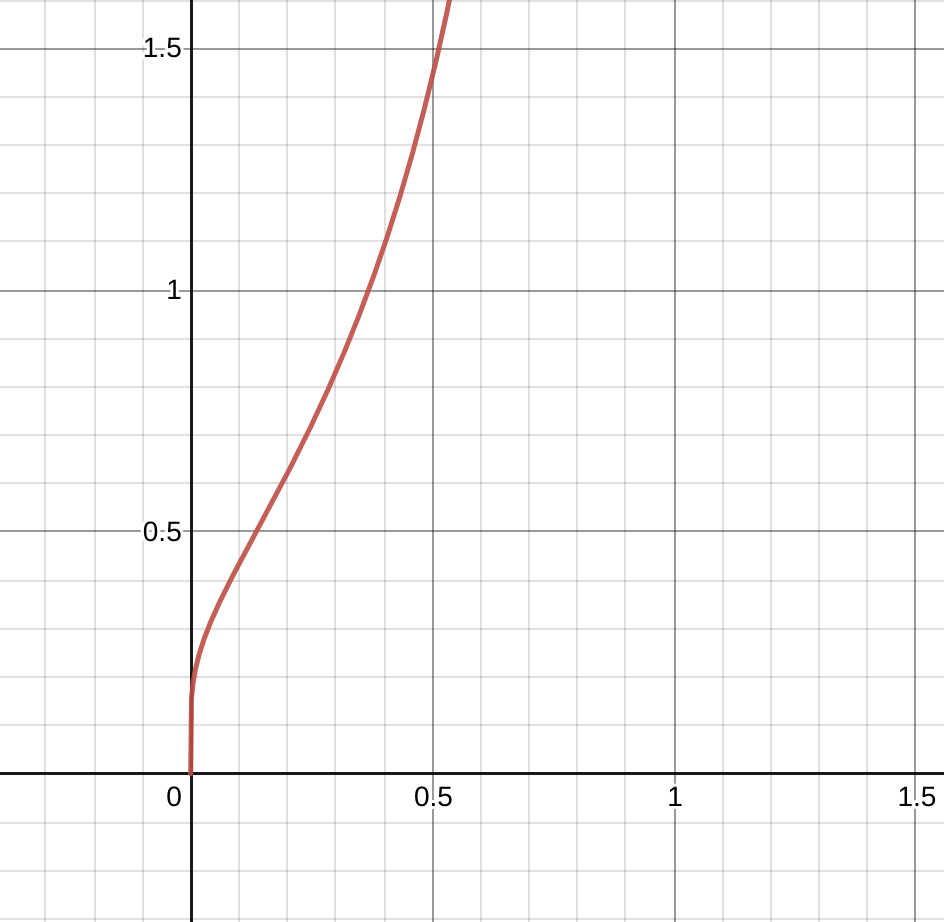
\includegraphics[width=\linewidth]{HMM_Only/function.png}
        \caption{Graph of the function $ y = \dfrac{-1}{ln(x)}$}
        \label{func}
        \end{subfigure}
        \begin{subfigure}{.45\textwidth}
        \centering
        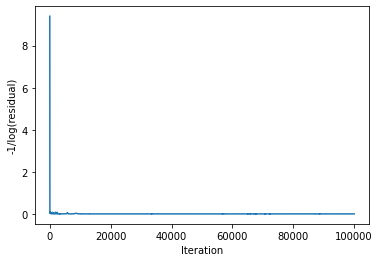
\includegraphics[width=\linewidth]{HMM_Only/convLog.png}
        \caption{Graph of function applied to residual of Baum-Welch against iteration number}
        \label{convlog}
        \end{subfigure}
        \caption{}
    \end{figure}

    The values decreases quite rapidly, thus to create a visual representation, we used the function $ y = \dfrac{-1}{ln(x)}$, where $x$ is the residual, to scale the values. We can see in Figure \ref{func} that our function is strictly increasing thus can be used for scaling. 

    Along with the CSV files containing the log, a graphical representation can be found in the Analysis Jupyter notebooks within each months folder. Figure \ref{convlog} shows one such graphical representation for the convergence log of attempt 1 for month 0. We can see that the residual converges to 0 relatively quickly, suggesting we could reduce the number of iterations. The convergence itself confirms that our two matrices and our initial distribution contain values close to the local optima. 

    \subsection{Selecting an Optimum}
    \label{Simple_Rainfall_HMM:Analysis:Selecting_an_Optimum}

    As mentioned earlier, we perform multiple random starts to try and obtain the global optimum. However, we do not know if it is the "most optimum" from the model alone. To do this, we count frequencies. 

    For each attempt, we count and record the frequency of occurrence of each integer in our observation set from our training rainfall data of 1000 observations as well as from our simulation generated by the HMM, also containing 1000 observations. We now find the difference between the two sets of frequencies, square the given value and then take a sum. The attempt the lowest sum of squares is then accepted as the most optimum optima. 

    For our example of month 0, we had the following results:
    \begin{center}
    \begin{tabular}{c c}
        Attempt & Sum of Square difference \\
        1 & 656 \\
        2 & 672 \\
        3 & 1692
    \end{tabular}
    \end{center}

    As such, we selected attempt 1 for our testing. The attempt selected for each month is in the below table.

    \begin{center}
    \begin{tabular}{c c c c c c c c c c c c c}
        Month   &  0  & 1 & 2 & 3 & 4 & 5 & 6 & 7 & 8 & 9 & 10 & 11 \\
        Attempt &  1  & 3 & 2 & 1 & 1 & 1 & 1 & 2 & 2 & 3 & 3  & 2 
    \end{tabular}  
    \end{center}

    \subsection{Results}
    \label{Simple_Rainfall_HMM:Analysis:Resutls}

    Since the results for each month are similar, we will only present results for month 0. The Results for other months can be found in the analysis files accompanying each months folder. 

    \begin{figure}
        \begin{subfigure}{.45\textwidth}
        \centering
        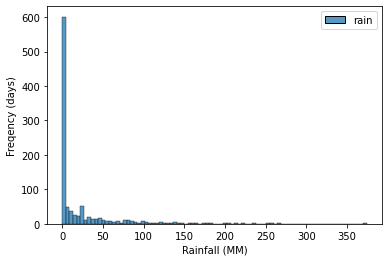
\includegraphics[width=\linewidth]{HMM_Only/0_freq_data.png}
        \caption{Observed Data}
        \label{inc0:data}
        \end{subfigure}
        \begin{subfigure}{.45\textwidth}
        \centering
        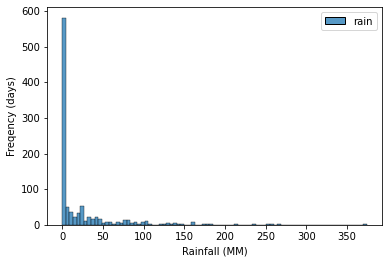
\includegraphics[width=\linewidth]{HMM_Only/0_freq_sim.png}
        \caption{Simulated Data}
        \label{inc0:sim}
        \end{subfigure}

        \begin{subfigure}{.45\textwidth}
        \centering
        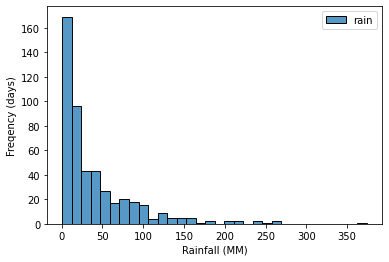
\includegraphics[width=\linewidth]{HMM_Only/_freq_data.png}
        \caption{Observed Data removing all 0mm days}
        \label{inc0:n0data}
        \end{subfigure}
        \begin{subfigure}{.45\textwidth}
        \centering
        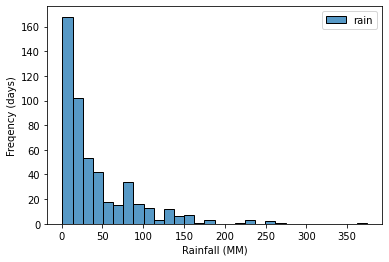
\includegraphics[width=\linewidth]{HMM_Only/_freq_sim.png}
        \caption{Simulated Data removing all 0mm days}
        \label{inc0:n0sim}
        \end{subfigure}
        \caption{Comparison of Observed data and Data simulated by HMM}
        \label{inc0}
    \end{figure}

    Figure \ref{inc0} shows that the frequencies seem to be similar for both simulations and recorded data. Furthermore, more minor details such as the peak at around 25mm also remains consistent. While this is promising, the large frequency for 0mm distorts the graph. To compare further, we plot the histograms once more, removing the first bar for 0mm. Here we can see it is not identical but seems to have similar properties, such as max, medium and high-density areas. We will investigate this result numerically in the results chapter of this paper.


    
	\newpage

	\chapter{Generalising the Observation Matrix}
	\label{Generalising_the_Observation_Matrix}
    In this chapter we will extend on Grando's ideas and adapt her model.


\section{Disk Structure}
Cowpertwait's disk structure for rain models is derived from nature. This makes it extremely appealing as a model. Giving Grando good reason to translate these ideas to her HMM based model. However, for our goal of rain simulation, her model has some unnessary complexity. 

Grando calculates the number of storm discs over the entire space (all sites) but then only selects discs above the current site. She repeats this for all sites. We can expect most storm discs will not cover all sites, suggesting this method will generate a large number of potential discs and then reject most of them. This is extremly ineffcient and computationaly expensive. To solve this issue one may propose the following:
\begin{itemize}
    \item Simulate the number and size of discs over the entire map of sites and deterimine which storms are above which sites. This method stops the unnessary iteration through all sites and provides the same results as the paramter estimates will be account for this change.
    \item Simulate the number and size of discs over all sites independently. Here we ignore the spatial data of the sites. This prevents us from understanding which sites are covered by the same discs, but this is not of importance to us and thus can be left as is. Furthermore, we can remove the assumption of the shape of the disc as it is no longer relevant, allowing our model to be further generalised. This allows us to remove the radius parameters for each state, reducing total parameters by the number of states.
\end{itemize}

While both methods mentioned above allow for improvement, ultimately it does not matter which we pick. The model will fit the given parameters and the orientation of the parameters does not make a difference as they will adjust to compensate, resulting in a model that produces a similar output. As such, for our model we decide to go with the second method. Since we will be calculating over each site independently, we decide to calculate parameters for each seperately rather than combining these results. 



\section{Split monthly}

Rainfall is not consistent throughout the year. A simulation of rainfall in summer would likely have signficiatnly different statistical properties to one from the winter. Grando's Model does not account for this, as such a simulation using this model could produce an output more likely in winter or summer, one cannot tell. 

To address these concerns, we utilise Cowpertwaits **ref** methodology, spliting the data into months. This allows for simulating for particular months as well as a better fit for the overall data. Since our data is a timeseries of rainfall amounts with not much other information given we divide our data into the average number of days in a month; 30. We then label the first twelve groups 0 to 11 and fill each group cyclying through 0-11. The exact methodology and jupyter notebook can be found in the "DataPrep" folder under "MyCode" within the code files. 

Another nessesary modeification was changing the missing values. The given data contained "-9999" for any days with missing data. Removing these values could create unequal sized datasets for each month. To avoid this we decided to set these values to a particular number. Unfortuently any value we select will cause the data mean to shift towards the value. To solve this we set this value as the mean of the months rainfall ignoring the missing data. 

\section{High dimensionality}

HMMs with even a few states contain a large number of paramters. Grando's Model contains 21. Through our adjustments made to the disc structure, we have reduced this to 18. High dimensionality is a common problem but Unfortuently does not have straightforward solutions. We could introduce new assumptions and try to simplify the data using dimensionality reduction methods but this may limit our ability to fit our model well. 

To address this problem, we revert back to chapter 4 \ref{chp4}. Instead of approaching this problem by starting the parameter estimation from the non-hmm parameters, we approach from HMM parameters. Momentarily ignoring the non-HMM paramters, we know that Baum-Welch can be used to estimate 12 of these 18 parameters. While this is not all, this is a great decrease in dimensions. However, our model does not have an observation matrix, which is required by the Baum-Welch **ref** algorithm. We address this in the following chapter.


	\newpage

	\chapter{Results}
    \label{Results}
	\section{Applying Baum Welch to Rainfall data}

\subsection{Building the Observation Matrix}

To be able to use Baum-Welch we require an observation probability matrix **ref**, thus in order to use it we must create one. To create a finite matrix of probabilities we require our data to be split into finite groups. Fortuantely the algorithm is increases in computation cost linearly with the dimensions of the observation matrix rather than squared as it does with the number of states. Through efficient implementation working with large observation matrices is feasible.

Through looking at the datasets, we can see the maximum rainfall is usually up to 1000mm. In our case this value was 743. Furthermore, the maximum precision of our data is integers. Thus, we can discretise our observations into integers up to the maximum rainfall for the given dataset. As we know from **ref**, the rows of the observation matrix represent the states and the columns represent the observations, giving us a matrix 3 by M matrix, where M is the number of observations.

We can now apply Baum-Welch to produce a HMM model that simulates integer values of daily rainfall in mm up to a given maximum amount. Code files can be found in "Baum Welch" folder under "MyCode". 

\begin{note}
    The values of the alpha and beta helper functions become extremly small for large sequence of observations. In our testing we found after about 1500 observations these values become too precise to store in "long double". This mathetmatically holds as the sum of the final alphas and betas represents the probability of observring the sequence **ref**, with a larger sequence the probability naturally decreases. We avoid this problem by using a sequence of 1000 observations. 
    
    When using this method, one must ensure the alpha and beta values are not all being stored as zeros.
\end{note}


\subsection{Local optimum vs global Optimum}

Once again from **ref**, we know that Baum-Welch converges to local optima. This suggests there may be a supperior optima, a superior fit for the model, that we have not found. To ensure a satisfactory fit is found, we repeat the algorithm for multiple random starts; random intial distribution, transition matrix and observation matrix. While this does not garentee we will find the global optima it reassures us that our given optima is farily suitable. 


We choose to do 3 attempts. This was an arbritaray choice. We recommend using a much larger number as we have selected this for simplicity of demonstration.


\section{Analysis}

The program "BaumWelch" requires the data split into months in csv files. For each month it outputs the fitted transition matrix, observation matrix, initial vector, a Convergence log and a simulation using the model. This is done over 12 threads, allocating one for each month. For our data we computed 100000 iterations of Baum-Welch. The three attempts took 1074.76, 1081.38 and 1076.16 seconds respectively.

\subsection{Convergence Log}

We introduced a Convergence log to ensure the algorithm did infact Converge. At each iteration, the difference between the current and previous transition matrix, observation matrix and intial distribution parameters was summed. This sum represent the residual, which we expect to tend to 0 as the number of iterations tends to $\infty$.

\begin{figure}
    \begin{subfigure}{.45\textwidth}
      \centering
      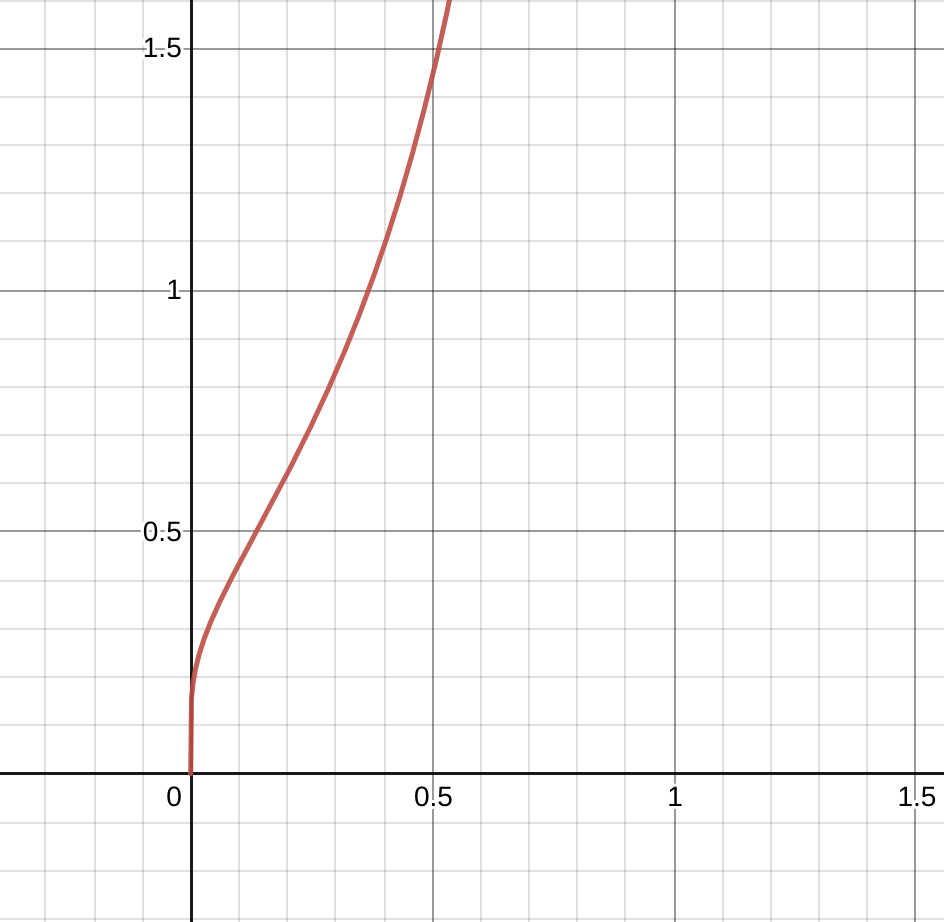
\includegraphics[width=\linewidth]{HMM_Only/function.png}
      \caption{}
      \label{func}
    \end{subfigure}
    \begin{subfigure}{.45\textwidth}
      \centering
      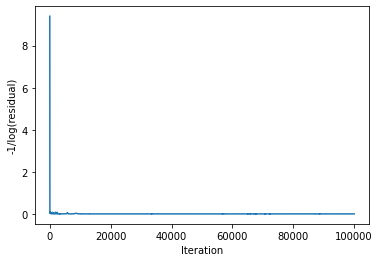
\includegraphics[width=\linewidth]{HMM_Only/convLog.png}
      \caption{}
      \label{convlog}
    \end{subfigure}
    \caption{}
\end{figure}

The values decrease quite rapidly, thus to create a visual representation we used the function $ y = \dfrac{-1}{ln(x)}$, where $x$ is the residual, to scale the values. We can see in Figure \ref{func} that our function is strictly increasing thus can be used for scaling. 

Along with the csv files containing the log, a graphical reprsentation can be found in the Analysis jupyter notebooks within each months folder. Figure \ref{convlog} shows one such graphical reprsentation for the covergence log of attempt 1 for month 0. We can see that the residual converges to 0 quite quickly, suggesting we could potentially reduce the number of iterations. The convergence itself confirms that the our two matrices and our intial distribution contain values close to the local optima. 





\subsection{Selecting the optimum optima}

As mentioned earlier, we perform multiple random starts to try and obtain the global optimum. However, from the model alone we do not know if it is the "most optimum". To do this we count frequencies. 

For each attempt we count and record the frequency of occurance of each interger in our observation set from our training rainfall data of 1000 observations as well as from our simulation generated by the HMM, also containing 1000 observations. We now find the difference the two sets of frequencies, square the given value and then take a sum. The attempt the lowest sum of squares is then accepted as the most optimum optima. 

For our example of month 0, we had the following results:
\begin{center}
  \begin{tabular}{c c}
    Attempt & Sum of Square difference \\
    1 & 656 \\
    2 & 672 \\
    3 & 1692
  \end{tabular}
\end{center}

As such we selected attempt 1 for our testing. The attempt selected for each month is given in below table.

\begin{center}
  \begin{tabular}{c c c c c c c c c c c c c}
    Month   &  0  & 1 & 2 & 3 & 4 & 5 & 6 & 7 & 8 & 9 & 10 & 11 \\
    Attempt &  1  & 3 & 2 & 1 & 1 & 1 & 1 & 2 & 2 & 3 & 3  & 2 
  \end{tabular}  
\end{center}

\subsection{Results}

Since the results for each month are quite similar , we will only present results for month 0. The Results for other months can be found in the analysis files accopymanying each months folder. 

\begin{figure}
    \begin{subfigure}{.45\textwidth}
      \centering
      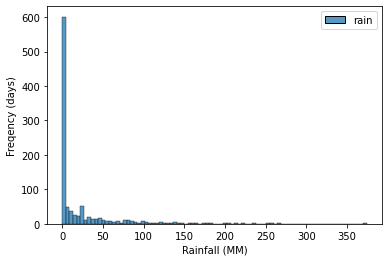
\includegraphics[width=\linewidth]{HMM_Only/0_freq_data.png}
      \caption{}
      \label{inc0:data}
    \end{subfigure}
    \begin{subfigure}{.45\textwidth}
      \centering
      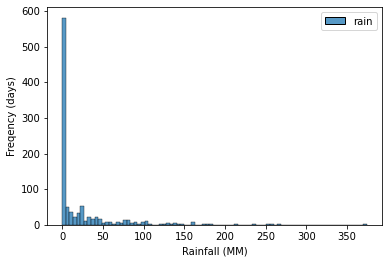
\includegraphics[width=\linewidth]{HMM_Only/0_freq_sim.png}
      \caption{}
      \label{inc0:sim}
    \end{subfigure}

    \begin{subfigure}{.45\textwidth}
      \centering
      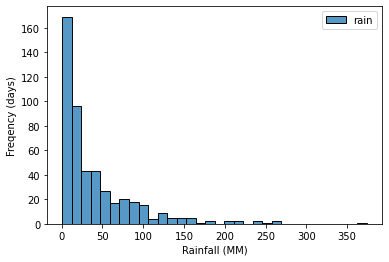
\includegraphics[width=\linewidth]{HMM_Only/_freq_data.png}
      \caption{}
      \label{inc0:n0data}
    \end{subfigure}
    \begin{subfigure}{.45\textwidth}
      \centering
      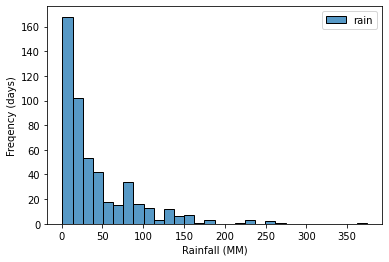
\includegraphics[width=\linewidth]{HMM_Only/_freq_sim.png}
      \caption{}
      \label{inc0:n0sim}
    \end{subfigure}
    \caption{}
    \label{inc0}
\end{figure}

From Figure \ref{inc0} we can see that the frequencies seem to be simliar for both simulation and recorded data. Furthermore, smaller details such as the peak at around 25mm also remains consitent. While this is promosing, the large frequency for 0mm distorts the graph. To compare further we plot the histograms once more, removing the first bar for 0mm. Here we can see it is not identical but seems to have similar properties, such as max, medium and high density areas. We will investigate this result numerically in the results chapter of this paper.



	\newpage

	\chapter{Future Research}
	\label{Future_Research}
    Our testing in \ref{Results} suggests the HMM on its own does have potential. The model matched both the training and test data well. While it did struggle to explain extreme rainfall, this could be an area for further research. Furthermore, for our testing, we used only three random starts of Baum-Welch. Considering the incredibly high complexity of the parameter space, due to large matrices, one can expect there to be many more local optima than just three. As such, increasing this number would likely increase the likelihood of achieving a better fit by finding a superior optimum.  Thus we are inclined to believe the performance of HMM rainfall models could be further improved.

Our generalised model was not successful. The model itself was chosen based on purely natural phenomenon and thus does not dismiss the idea that a generalised HMM model may be helpful. If we can find a function of random variables that perfectly fit the rows of the observation matrix, then hypothetically, we can expect matching performance to that of the HMM only model.  While the HMM fits the observed data more closely, a generalised model will likely allow for improvements in out-of-sample testing, particularly at the extremes. 

We tested a three-state model. However, this was an arbitrary choice. Future research may consider increasing this number as it may allow for a superior fit to the data. This change, of course, must be done after careful considerations of computational cost as the algorithms used in fitting are extremely sensitive to the increase in value of this parameter.

To conclude, can hidden Markov models be used to simulate rainfall? From our testing, we have insufficient evidence to suggest not. Further research into the three areas listed above combined with testing performance against other models should determine whether HMMs provide any advantage.
	\newpage

	\nocite{*}
	\printbibliography

\end{document}